\documentclass[twoside]{book}

% Packages required by doxygen
\usepackage{fixltx2e}
\usepackage{calc}
\usepackage{doxygen}
\usepackage[export]{adjustbox} % also loads graphicx
\usepackage{graphicx}
\usepackage[utf8]{inputenc}
\usepackage{makeidx}
\usepackage{multicol}
\usepackage{multirow}
\PassOptionsToPackage{warn}{textcomp}
\usepackage{textcomp}
\usepackage[nointegrals]{wasysym}
\usepackage[table]{xcolor}

% Font selection
\usepackage[T1]{fontenc}
\usepackage[scaled=.90]{helvet}
\usepackage{courier}
\usepackage{amssymb}
\usepackage{sectsty}
\renewcommand{\familydefault}{\sfdefault}
\allsectionsfont{%
  \fontseries{bc}\selectfont%
  \color{darkgray}%
}
\renewcommand{\DoxyLabelFont}{%
  \fontseries{bc}\selectfont%
  \color{darkgray}%
}
\newcommand{\+}{\discretionary{\mbox{\scriptsize$\hookleftarrow$}}{}{}}

% Page & text layout
\usepackage{geometry}
\geometry{%
  a4paper,%
  top=2.5cm,%
  bottom=2.5cm,%
  left=2.5cm,%
  right=2.5cm%
}
\tolerance=750
\hfuzz=15pt
\hbadness=750
\setlength{\emergencystretch}{15pt}
\setlength{\parindent}{0cm}
\setlength{\parskip}{3ex plus 2ex minus 2ex}
\makeatletter
\renewcommand{\paragraph}{%
  \@startsection{paragraph}{4}{0ex}{-1.0ex}{1.0ex}{%
    \normalfont\normalsize\bfseries\SS@parafont%
  }%
}
\renewcommand{\subparagraph}{%
  \@startsection{subparagraph}{5}{0ex}{-1.0ex}{1.0ex}{%
    \normalfont\normalsize\bfseries\SS@subparafont%
  }%
}
\makeatother

% Headers & footers
\usepackage{fancyhdr}
\pagestyle{fancyplain}
\fancyhead[LE]{\fancyplain{}{\bfseries\thepage}}
\fancyhead[CE]{\fancyplain{}{}}
\fancyhead[RE]{\fancyplain{}{\bfseries\leftmark}}
\fancyhead[LO]{\fancyplain{}{\bfseries\rightmark}}
\fancyhead[CO]{\fancyplain{}{}}
\fancyhead[RO]{\fancyplain{}{\bfseries\thepage}}
\fancyfoot[LE]{\fancyplain{}{}}
\fancyfoot[CE]{\fancyplain{}{}}
\fancyfoot[RE]{\fancyplain{}{\bfseries\scriptsize Generated by Doxygen }}
\fancyfoot[LO]{\fancyplain{}{\bfseries\scriptsize Generated by Doxygen }}
\fancyfoot[CO]{\fancyplain{}{}}
\fancyfoot[RO]{\fancyplain{}{}}
\renewcommand{\footrulewidth}{0.4pt}
\renewcommand{\chaptermark}[1]{%
  \markboth{#1}{}%
}
\renewcommand{\sectionmark}[1]{%
  \markright{\thesection\ #1}%
}

% Indices & bibliography
\usepackage{natbib}
\usepackage[titles]{tocloft}
\setcounter{tocdepth}{3}
\setcounter{secnumdepth}{5}
\makeindex

% Hyperlinks (required, but should be loaded last)
\usepackage{ifpdf}
\ifpdf
  \usepackage[pdftex,pagebackref=true]{hyperref}
\else
  \usepackage[ps2pdf,pagebackref=true]{hyperref}
\fi
\hypersetup{%
  colorlinks=true,%
  linkcolor=blue,%
  citecolor=blue,%
  unicode%
}

% Custom commands
\newcommand{\clearemptydoublepage}{%
  \newpage{\pagestyle{empty}\cleardoublepage}%
}

\usepackage{caption}
\captionsetup{labelsep=space,justification=centering,font={bf},singlelinecheck=off,skip=4pt,position=top}

%===== C O N T E N T S =====

\begin{document}

% Titlepage & ToC
\hypersetup{pageanchor=false,
             bookmarksnumbered=true,
             pdfencoding=unicode
            }
\pagenumbering{alph}
\begin{titlepage}
\vspace*{7cm}
\begin{center}%
{\Large My Project }\\
\vspace*{1cm}
{\large Generated by Doxygen 1.8.13}\\
\end{center}
\end{titlepage}
\clearemptydoublepage
\pagenumbering{roman}
\tableofcontents
\clearemptydoublepage
\pagenumbering{arabic}
\hypersetup{pageanchor=true}

%--- Begin generated contents ---
\chapter{Hierarchical Index}
\doxysection{Class Hierarchy}
This inheritance list is sorted roughly, but not completely, alphabetically\+:\begin{DoxyCompactList}
\item \contentsline{section}{Controller}{\pageref{classController}}{}
\item \contentsline{section}{Document}{\pageref{classDocument}}{}
\item \contentsline{section}{Model}{\pageref{classModel}}{}
\item \contentsline{section}{Shape}{\pageref{classShape}}{}
\begin{DoxyCompactList}
\item \contentsline{section}{Circle}{\pageref{classCircle}}{}
\item \contentsline{section}{Square}{\pageref{classSquare}}{}
\end{DoxyCompactList}
\item \contentsline{section}{View}{\pageref{classView}}{}
\end{DoxyCompactList}

\chapter{Class Index}
\doxysection{Class List}
Here are the classes, structs, unions and interfaces with brief descriptions\+:\begin{DoxyCompactList}
\item\contentsline{section}{\mbox{\hyperlink{classCanvas}{Canvas}} }{\pageref{classCanvas}}{}
\item\contentsline{section}{\mbox{\hyperlink{classCanvasClick}{Canvas\+Click}} }{\pageref{classCanvasClick}}{}
\item\contentsline{section}{\mbox{\hyperlink{classCanvasInfo}{Canvas\+Info}} }{\pageref{classCanvasInfo}}{}
\item\contentsline{section}{\mbox{\hyperlink{classCanvasLayer}{Canvas\+Layer}} }{\pageref{classCanvasLayer}}{}
\item\contentsline{section}{\mbox{\hyperlink{classCanvasMouseMove}{Canvas\+Mouse\+Move}} }{\pageref{classCanvasMouseMove}}{}
\item\contentsline{section}{\mbox{\hyperlink{classController}{Controller}} }{\pageref{classController}}{}
\item\contentsline{section}{\mbox{\hyperlink{classCreateSquareButton}{Create\+Square\+Button}} }{\pageref{classCreateSquareButton}}{}
\item\contentsline{section}{\mbox{\hyperlink{classCreateTriangleButton}{Create\+Triangle\+Button}} }{\pageref{classCreateTriangleButton}}{}
\item\contentsline{section}{\mbox{\hyperlink{classEmptyEvent}{Empty\+Event}} }{\pageref{classEmptyEvent}}{}
\item\contentsline{section}{\mbox{\hyperlink{classExportButton}{Export\+Button}} }{\pageref{classExportButton}}{}
\item\contentsline{section}{\mbox{\hyperlink{classGUI}{GUI}} }{\pageref{classGUI}}{}
\item\contentsline{section}{\mbox{\hyperlink{classHardwareObjects}{Hardware\+Objects}} }{\pageref{classHardwareObjects}}{}
\item\contentsline{section}{\mbox{\hyperlink{classImportButton}{Import\+Button}} }{\pageref{classImportButton}}{}
\item\contentsline{section}{\mbox{\hyperlink{classKeyboard}{Keyboard}} }{\pageref{classKeyboard}}{}
\item\contentsline{section}{\mbox{\hyperlink{classKeyboardEvent}{Keyboard\+Event}} }{\pageref{classKeyboardEvent}}{}
\item\contentsline{section}{\mbox{\hyperlink{classKeyboardWidget}{Keyboard\+Widget}} }{\pageref{classKeyboardWidget}}{}
\item\contentsline{section}{\mbox{\hyperlink{classLoadButtonClick}{Load\+Button\+Click}} }{\pageref{classLoadButtonClick}}{}
\item\contentsline{section}{\mbox{\hyperlink{classModel}{Model}} }{\pageref{classModel}}{}
\item\contentsline{section}{\mbox{\hyperlink{classMouse}{Mouse}} }{\pageref{classMouse}}{}
\item\contentsline{section}{\mbox{\hyperlink{structPoint}{Point}} }{\pageref{structPoint}}{}
\item\contentsline{section}{\mbox{\hyperlink{structRectangle}{Rectangle}} }{\pageref{structRectangle}}{}
\item\contentsline{section}{\mbox{\hyperlink{classSaveButton}{Save\+Button}} }{\pageref{classSaveButton}}{}
\item\contentsline{section}{\mbox{\hyperlink{classSaveButtonClick}{Save\+Button\+Click}} }{\pageref{classSaveButtonClick}}{}
\item\contentsline{section}{\mbox{\hyperlink{structShape}{Shape}} }{\pageref{structShape}}{}
\item\contentsline{section}{\mbox{\hyperlink{classState}{State}} }{\pageref{classState}}{}
\item\contentsline{section}{\mbox{\hyperlink{classUserClick}{User\+Click}} }{\pageref{classUserClick}}{}
\item\contentsline{section}{\mbox{\hyperlink{classUserEvent}{User\+Event}} }{\pageref{classUserEvent}}{}
\item\contentsline{section}{\mbox{\hyperlink{classUserInfo}{User\+Info}} }{\pageref{classUserInfo}}{}
\item\contentsline{section}{\mbox{\hyperlink{classUserMouseMove}{User\+Mouse\+Move}} }{\pageref{classUserMouseMove}}{}
\item\contentsline{section}{\mbox{\hyperlink{classWidget}{Widget}} }{\pageref{classWidget}}{}
\end{DoxyCompactList}

\chapter{Class Documentation}
\hypertarget{classCircle}{}\section{Circle Class Reference}
\label{classCircle}\index{Circle@{Circle}}


Inheritance diagram for Circle\+:
\nopagebreak
\begin{figure}[H]
\begin{center}
\leavevmode
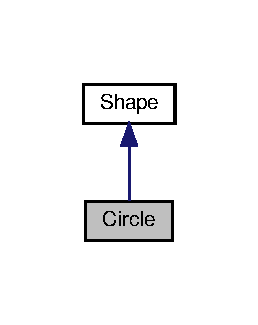
\includegraphics[width=124pt]{classCircle__inherit__graph}
\end{center}
\end{figure}


Collaboration diagram for Circle\+:
\nopagebreak
\begin{figure}[H]
\begin{center}
\leavevmode
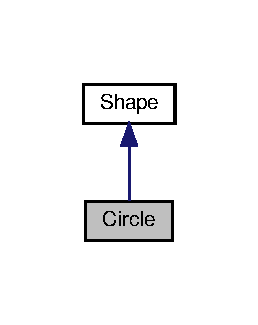
\includegraphics[width=124pt]{classCircle__coll__graph}
\end{center}
\end{figure}
\subsection*{Public Member Functions}
\begin{DoxyCompactItemize}
\item 
\mbox{\Hypertarget{classCircle_a694e0245495333f2e22c78a6ec4431e2}\label{classCircle_a694e0245495333f2e22c78a6ec4431e2}} 
void {\bfseries Request\+Params} ()
\item 
\mbox{\Hypertarget{classCircle_a69f872d104bce615dd56eb2b5c87d224}\label{classCircle_a69f872d104bce615dd56eb2b5c87d224}} 
Shape\+Type {\bfseries My\+Type} ()
\end{DoxyCompactItemize}


The documentation for this class was generated from the following file\+:\begin{DoxyCompactItemize}
\item 
Shape.\+h\end{DoxyCompactItemize}

\hypertarget{classController}{}\doxysection{Controller Class Reference}
\label{classController}\index{Controller@{Controller}}
\doxysubsection*{Public Member Functions}
\begin{DoxyCompactItemize}
\item 
\mbox{\Hypertarget{classController_a7dbaa458c5c4a836a697c54fb4d34508}\label{classController_a7dbaa458c5c4a836a697c54fb4d34508}} 
void {\bfseries Finish\+Event\+Sequence} ()
\item 
\mbox{\Hypertarget{classController_a4c94bfb506699fea0583f7c92b084399}\label{classController_a4c94bfb506699fea0583f7c92b084399}} 
bool {\bfseries Manage} (\mbox{\hyperlink{classUserEvent}{User\+Event}} $\ast$e, \mbox{\hyperlink{classModel}{Model}} \&mod, \mbox{\hyperlink{classGUI}{GUI}} \&ui)
\end{DoxyCompactItemize}


The documentation for this class was generated from the following files\+:\begin{DoxyCompactItemize}
\item 
Controller.\+h\item 
Controller.\+cpp\end{DoxyCompactItemize}

\hypertarget{classDocument}{}\doxysection{Document Class Reference}
\label{classDocument}\index{Document@{Document}}
\doxysubsection*{Public Member Functions}
\begin{DoxyCompactItemize}
\item 
\mbox{\Hypertarget{classDocument_a3edd06d81e5d1f87564c930dbe0d1316}\label{classDocument_a3edd06d81e5d1f87564c930dbe0d1316}} 
{\bfseries Document} (string name)
\item 
\mbox{\Hypertarget{classDocument_afd8d9bdd8b2936379bc22dd803b8e17d}\label{classDocument_afd8d9bdd8b2936379bc22dd803b8e17d}} 
string {\bfseries Get\+Name} ()
\item 
\mbox{\Hypertarget{classDocument_a096f0a4079dc0c198f03b44b73a2459e}\label{classDocument_a096f0a4079dc0c198f03b44b73a2459e}} 
void {\bfseries Set\+Id} (int id)
\item 
\mbox{\Hypertarget{classDocument_afa5eddc4bc257ce632aa408ead1c67d4}\label{classDocument_afa5eddc4bc257ce632aa408ead1c67d4}} 
int {\bfseries Get\+Id} ()
\item 
\mbox{\Hypertarget{classDocument_a521cf739e7cc9cb16a45cce98073b697}\label{classDocument_a521cf739e7cc9cb16a45cce98073b697}} 
void {\bfseries Add\+Shape} (\mbox{\hyperlink{classShape}{Shape}} $\ast$sh)
\item 
\mbox{\Hypertarget{classDocument_a4b30fd9612a3c84e2fff345e46d094c8}\label{classDocument_a4b30fd9612a3c84e2fff345e46d094c8}} 
bool {\bfseries Delete\+Shape} (int id)
\end{DoxyCompactItemize}


The documentation for this class was generated from the following file\+:\begin{DoxyCompactItemize}
\item 
Model.\+h\end{DoxyCompactItemize}

\hypertarget{classModel}{}\section{Model Class Reference}
\label{classModel}\index{Model@{Model}}
\subsection*{Public Member Functions}
\begin{DoxyCompactItemize}
\item 
\mbox{\Hypertarget{classModel_a00377628187a30d8232110df56d15771}\label{classModel_a00377628187a30d8232110df56d15771}} 
void {\bfseries Save\+State\+To\+File} (std\+::string filename)
\item 
\mbox{\Hypertarget{classModel_a64abdebeccd4fcd19d41a14d87aeebd5}\label{classModel_a64abdebeccd4fcd19d41a14d87aeebd5}} 
void {\bfseries Load\+State\+From\+File} (std\+::string filename)
\item 
\mbox{\Hypertarget{classModel_a5842c35a0dda88f6c0bd1e5f8a1ed404}\label{classModel_a5842c35a0dda88f6c0bd1e5f8a1ed404}} 
void {\bfseries Go\+Back\+To\+Previous\+State} ()
\item 
\mbox{\Hypertarget{classModel_a1bc43dc264d3772403975d8e1955ddb0}\label{classModel_a1bc43dc264d3772403975d8e1955ddb0}} 
bool {\bfseries Attach\+State} (\hyperlink{classState}{State} \&s)
\end{DoxyCompactItemize}


The documentation for this class was generated from the following file\+:\begin{DoxyCompactItemize}
\item 
Model.\+h\end{DoxyCompactItemize}

\hypertarget{classShape}{}\section{Shape Class Reference}
\label{classShape}\index{Shape@{Shape}}


Inheritance diagram for Shape\+:
\nopagebreak
\begin{figure}[H]
\begin{center}
\leavevmode
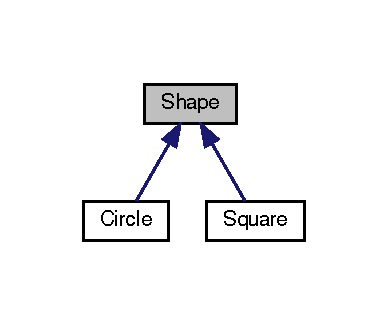
\includegraphics[width=188pt]{classShape__inherit__graph}
\end{center}
\end{figure}
\subsection*{Public Member Functions}
\begin{DoxyCompactItemize}
\item 
\mbox{\Hypertarget{classShape_a677f57ffcd291adc2fe1bb884cd80576}\label{classShape_a677f57ffcd291adc2fe1bb884cd80576}} 
virtual void {\bfseries Request\+Params} ()
\item 
\mbox{\Hypertarget{classShape_ae80ee2a092e3042b0ccaa2c7dcf6e04b}\label{classShape_ae80ee2a092e3042b0ccaa2c7dcf6e04b}} 
void {\bfseries Set\+Id} (int id)
\item 
\mbox{\Hypertarget{classShape_a619cb49e2f5acdbecf216f262fa2a85f}\label{classShape_a619cb49e2f5acdbecf216f262fa2a85f}} 
int {\bfseries Get\+Id} ()
\end{DoxyCompactItemize}


The documentation for this class was generated from the following file\+:\begin{DoxyCompactItemize}
\item 
Shape.\+h\end{DoxyCompactItemize}

\hypertarget{classSquare}{}\section{Square Class Reference}
\label{classSquare}\index{Square@{Square}}


Inheritance diagram for Square\+:
\nopagebreak
\begin{figure}[H]
\begin{center}
\leavevmode
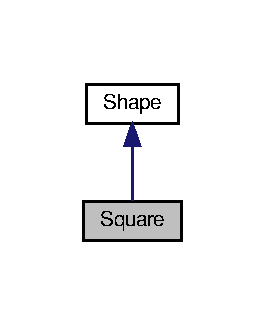
\includegraphics[width=127pt]{classSquare__inherit__graph}
\end{center}
\end{figure}


Collaboration diagram for Square\+:
\nopagebreak
\begin{figure}[H]
\begin{center}
\leavevmode
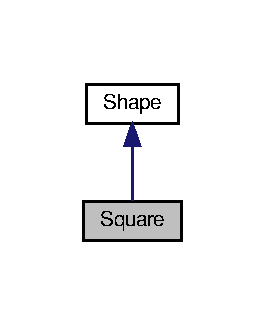
\includegraphics[width=127pt]{classSquare__coll__graph}
\end{center}
\end{figure}
\subsection*{Public Member Functions}
\begin{DoxyCompactItemize}
\item 
\mbox{\Hypertarget{classSquare_ae1640c4edbcf409671b230a405a707e2}\label{classSquare_ae1640c4edbcf409671b230a405a707e2}} 
void {\bfseries Request\+Params} ()
\item 
\mbox{\Hypertarget{classSquare_a6ce99af81c134404c21e15e1cfbe5664}\label{classSquare_a6ce99af81c134404c21e15e1cfbe5664}} 
Shape\+Type {\bfseries My\+Type} ()
\end{DoxyCompactItemize}


The documentation for this class was generated from the following file\+:\begin{DoxyCompactItemize}
\item 
Shape.\+h\end{DoxyCompactItemize}

\hypertarget{classView}{}\doxysection{View Class Reference}
\label{classView}\index{View@{View}}
\doxysubsection*{Public Member Functions}
\begin{DoxyCompactItemize}
\item 
\mbox{\Hypertarget{classView_aad48b922cbd2efb97313d597a088ce2a}\label{classView_aad48b922cbd2efb97313d597a088ce2a}} 
void {\bfseries Event\+Listener} ()
\end{DoxyCompactItemize}


The documentation for this class was generated from the following file\+:\begin{DoxyCompactItemize}
\item 
View.\+h\end{DoxyCompactItemize}

%--- End generated contents ---

% Index
\backmatter
\newpage
\phantomsection
\clearemptydoublepage
\addcontentsline{toc}{chapter}{Index}
\printindex

\end{document}
